\section {Desarrollo}

En esta sección se va describir las diferentes tareas que se han realizado para diseñar una posible solución de la práctica.

\subsection{Lectura y escritura CSV}
Para la lectura y escritura de datos en archivos utilizaremos una tarjeta microSD compatible con nuestro arduino UNO, será la encargada de registrar los datos recogidos por los sensores. Para poder utilizarla en el arduino se debe conectar según el siguiente esquema:
\begin{enumerate} 
    \item \textbf{CS (Chip Select)}: Para seleccionar la tarjeta SD al comunicar.
    \item \textbf{DI (Data In)}: Para mandar datos desde el arduino a la SD. 
    \item \textbf{DO (Data Out)}:Para recibir datos desde la SD al arduino. 
    \item \textbf{SCK (Serial Clock)}: Proporciona la señal de reloj para sincronizar la comunicación de datos. 
    \item \textbf{VCC}: Para dar energía a la SD. 
    \item \textbf{GND}: Para cerrar el circuit.
\end{enumerate}

\begin{figure}[H]
    \centering
    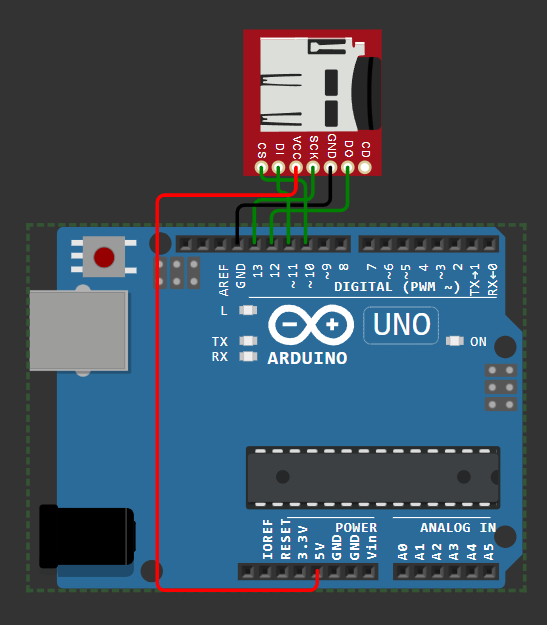
\includegraphics[width = 10cm]{ImagenesLatex/microsd.PNG}{}
    \caption{MicroSD}
    % \label{fig:enter-label}
\end{figure}

Una vez creado el circuito, podemos implementar la lógica en código que permita crear un archivo .csv y manipularlo:
\begin{enumerate}

    \item Iniciar comunicación Serial: esto es necesario ya que se va a utilizar la plataforma Wokwi, en vez de acceder a una tarjeta física real. Utilizaremos esta comunicación para mostrar los resultados así como el contenido de la tarjeta SD tras escritura.  

    \item Abrir el archivo csv: esto se realiza mediante el uso de la librería SD. Se puede abrir en modo lectura o escritura, y se debe cerrar al final.
    
    \item Escritura de datos: se escribe a modo de prueba inicial solo la cabecera del archivo.

    \item Lectura: se abre para lectura y se comprueba que se ha añadido una cabecera correctamente.

\end{enumerate}

\begin{figure}[H]
    \centering
    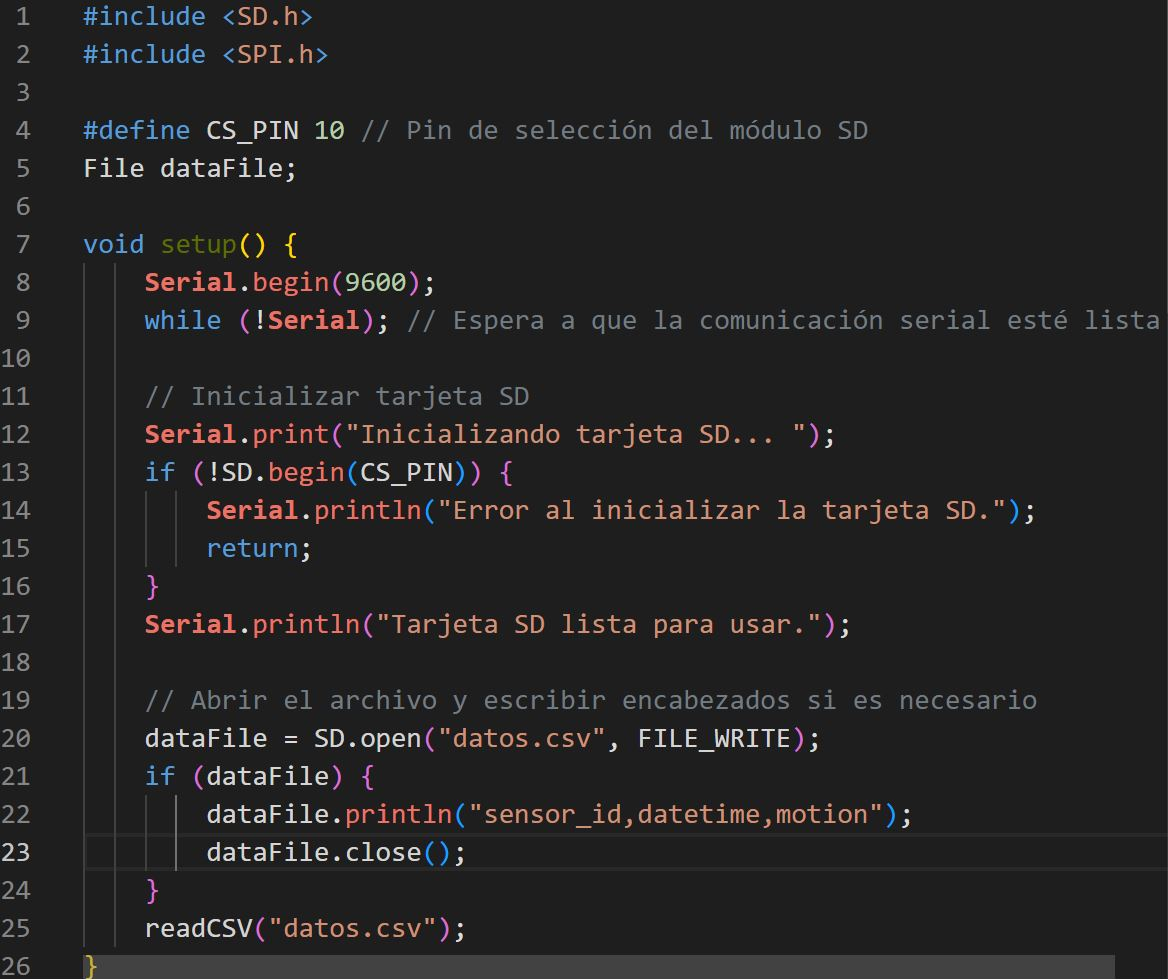
\includegraphics[width = 10cm]{ImagenesLatex/csv_header.JPG}{}
    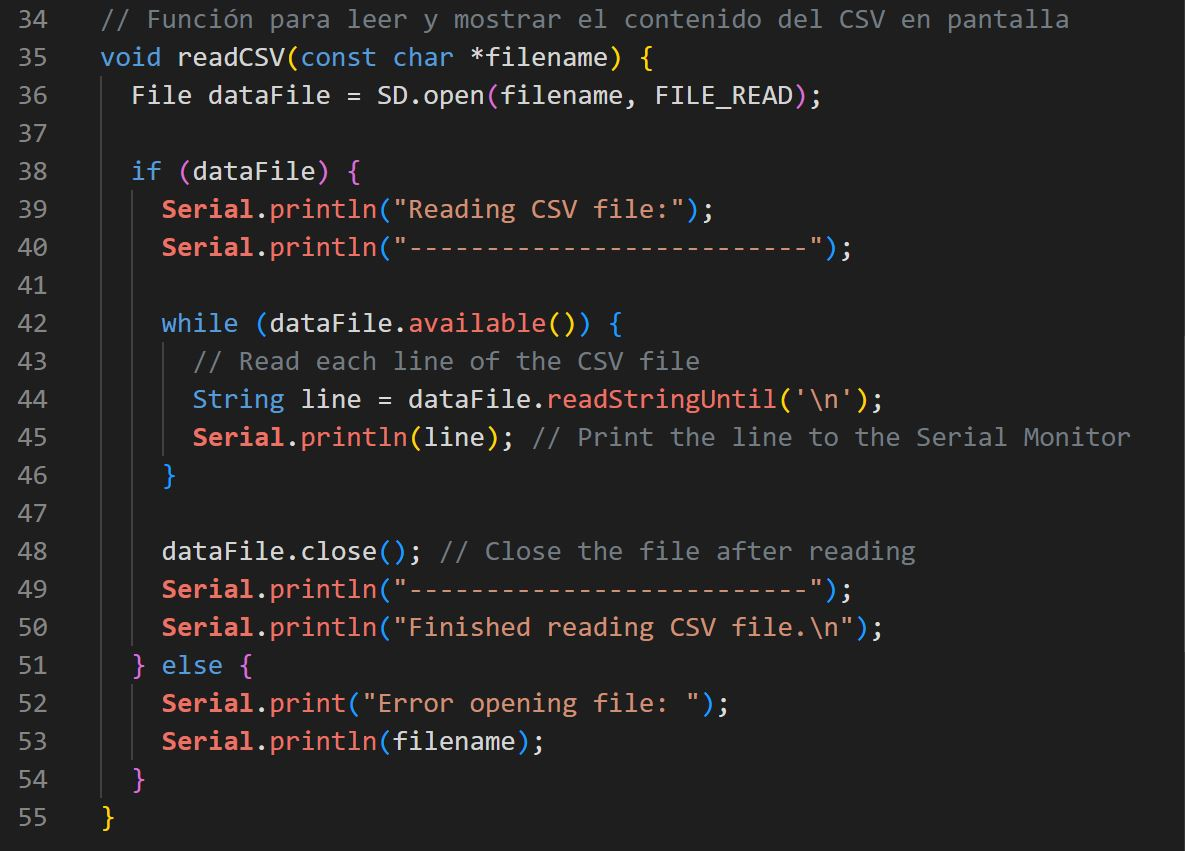
\includegraphics[width = 10cm]{ImagenesLatex/csv_header_read.JPG}{}
    \caption{Escritura y lectura SD}
    % \label{fig:enter-label}
\end{figure}

Finalmente podemos utilizar el Serial display para comprobar que hemos añadido la cabecera correctamente.


\begin{figure}[H]
    \centering
    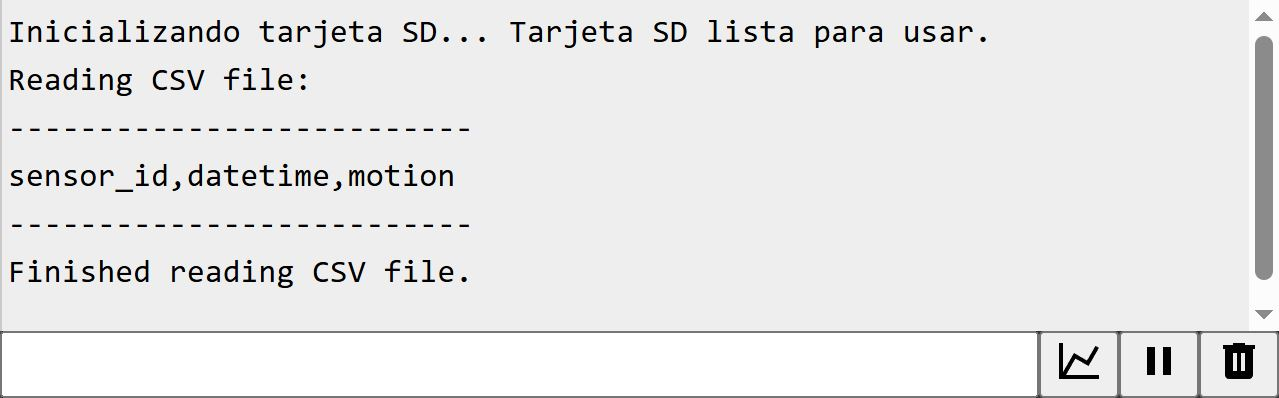
\includegraphics[width = 10cm]{ImagenesLatex/res_csv_header.JPG}{}
    \caption{Serial display}
    % \label{fig:enter-label}
\end{figure}


\subsection{Sensor de movimiento PIR}
En este ejercicio se propone el uso de un sensor de movimiento, utilizaremos sensores PIR. El esquema de pines para el sensor es el siguiente:
\begin{enumerate}
    \item Polo negativo: Se conectará a un voltaje de 5V.
    \item Polo positivo: Se conectara a GND para cerrar el circuito.
    \item Pin de lectura: Se conectará a un pin que permita lectura digital.
\end{enumerate}

\begin{figure}[H]
    \centering
    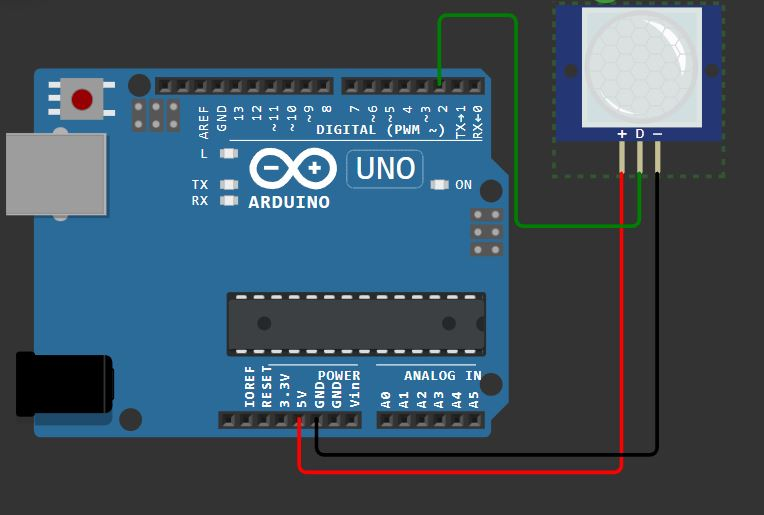
\includegraphics[width = 10cm]{ImagenesLatex/pir.JPG}{}
    \caption{Sensor PIR}
    % \label{fig:enter-label}
\end{figure}

Simplemente con la función digitalRead podremos obtener si existe movimiento o no. A continuación se muestra un ejemplo de uso:

\begin{figure}[H]
    \centering
    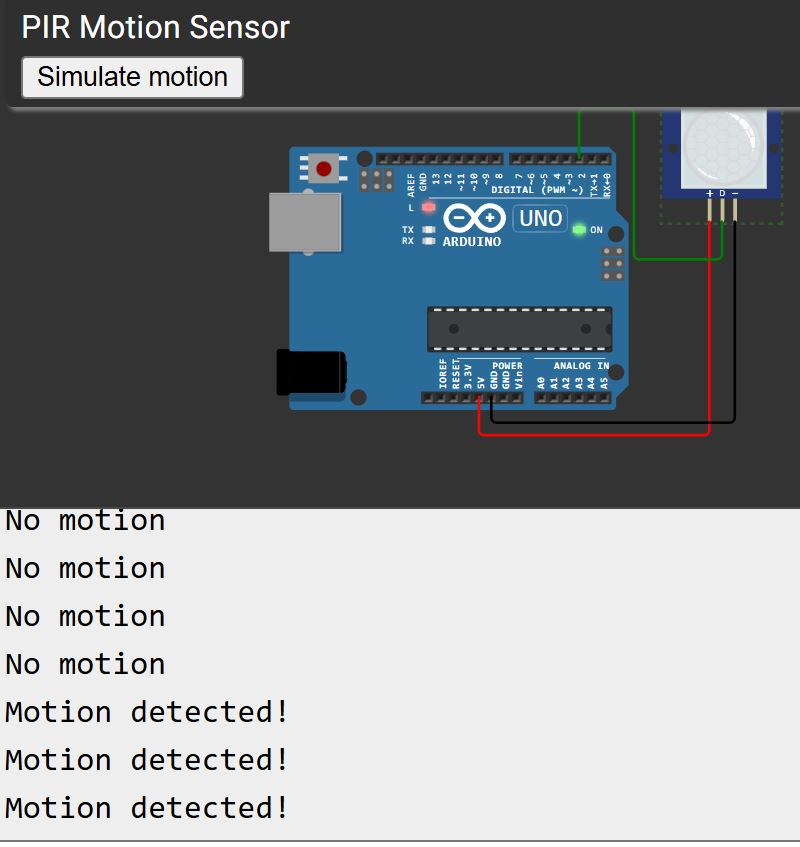
\includegraphics[width = 10cm]{ImagenesLatex/pir_simulation.JPG}{}
    \caption{Simulación sensor PIR}
    % \label{fig:enter-label}
\end{figure}

El simulador de Wokwi nos permite simular movimiento en el sensor, que podemos reflejar utilizando digitalRead en combinación con el display serial.

\subsection{Fecha y hora con RTC}
Para obtener la fecha hora y poder dar un sentido temporal a los datos de nuestros sensores utilizaremos un módulo de reloj en tiempo real llamado DS1307 RTC. El esquema de pines que sigue el circuito es el siguiente:
\begin{enumerate}
    \item Pin de voltaje: Se conectará con un voltaje de 5V.
    \item Pin de GND: Se conectara a GND para cerrar el circuito.
    \item Pin SDA (Serial Data): Se conectará con un pin analógico.
    \item Pin SCL (Serial Clock): Se conectará con un pin analógico. 
\end{enumerate}
Nótese que los pines SDA y SCL se utilizan para la comunicación entre arduino y el realtime clock. El circuito queda como sigue:

\begin{figure}[H]
    \centering
    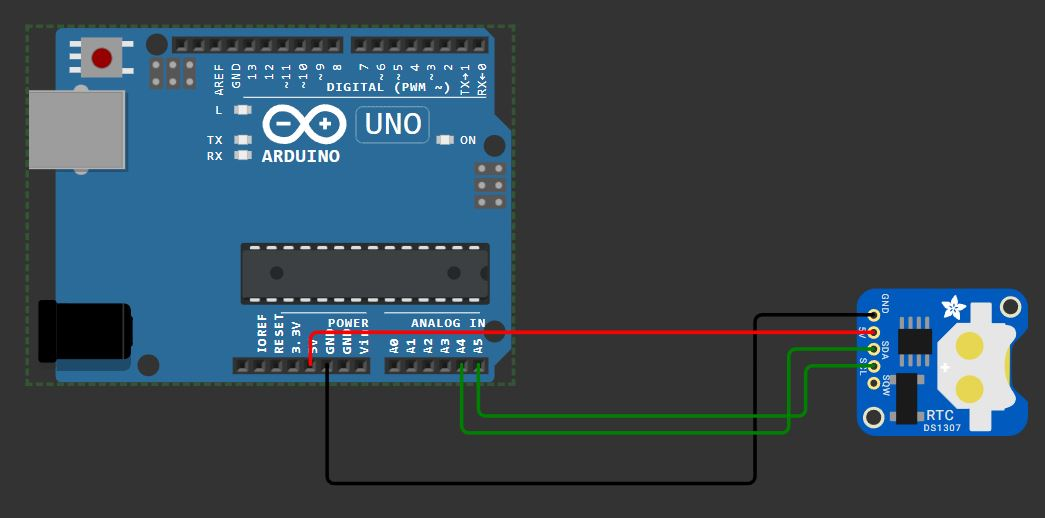
\includegraphics[width = 10cm]{ImagenesLatex/rtc_circuit.JPG}{}
    \caption{Simulación sensor PIR}
    % \label{fig:enter-label}
\end{figure}

A continuación se muestra como se extrae del objeto DateTime el valor de la fecha y la hora:
\begin{figure}[H]
    \centering
    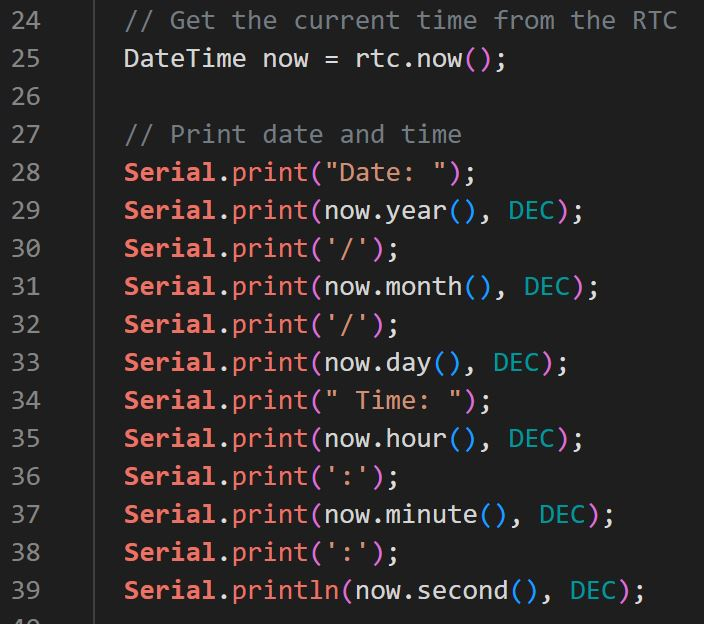
\includegraphics[width = 10cm]{ImagenesLatex/code_rtc.JPG}{}
    \caption{Simulación sensor PIR}
    % \label{fig:enter-label}
\end{figure}

En este caso se hace print a la comunicación Serial, pero podemos utilizar cualquier medio de comunicación, como por ejemplo a la tarjeta SD de manera que se puedan guardar las fechas (y otros datos) de forma persistente.

Finalmente se simula el uso del RTC:

\begin{figure}[H]
    \centering
    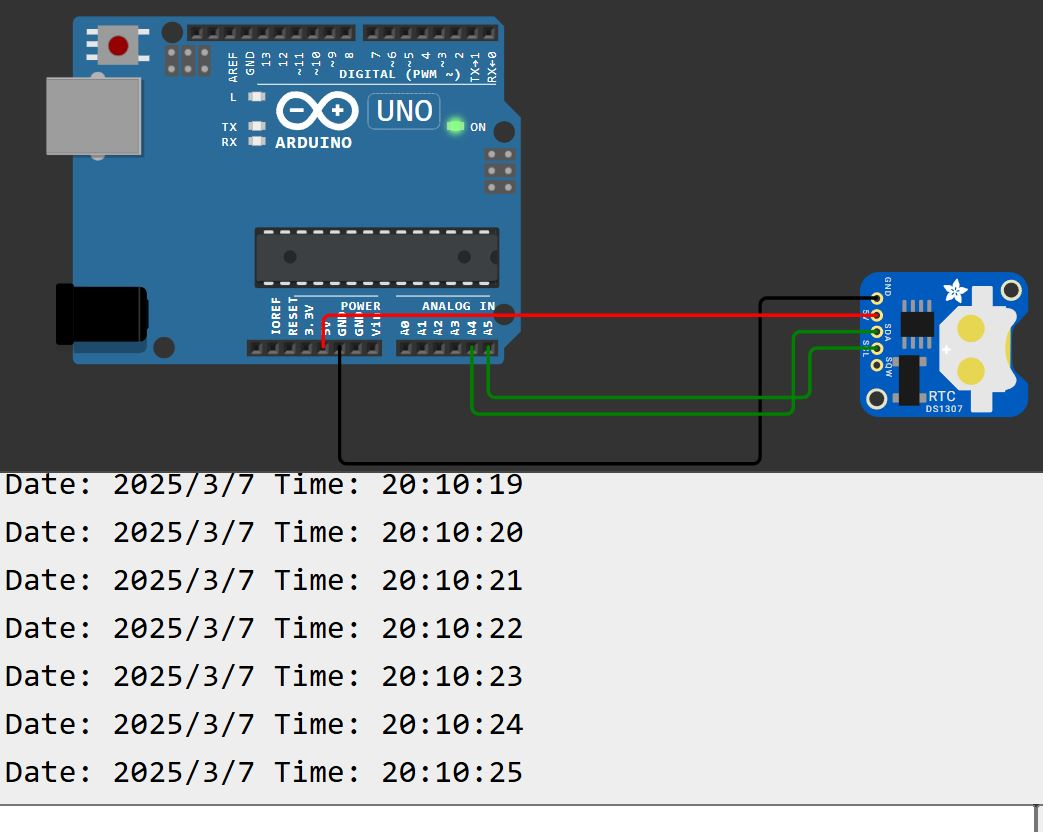
\includegraphics[width = 10cm]{ImagenesLatex/rtc.JPG}{}
    \caption{Simulación sensor PIR}
    % \label{fig:enter-label}
\end{figure}

\subsection{Integración 4 sensores con tiempo y registro en SD}
Finalmente, podemos agrupar los elementos vistos anteriormente para resolver el ejercicio pedido. En resumen, nuestro circuito constará de los siguientes elementos:
\begin{enumerate}
    \item Dispositivo Iot: Arduino UNO para la integración de los elementos y su comunicación.
    \item Tarjeta SD: MicroSD para el almacenamiento de los datos.
    \item Sensores: 4 sensores de tipo PIR que registran movimiento en formato digital, esto es, uno o cero.
    \item Reloj: Módulo de reloj DS1307 para el registro de la fecha y la hora.
\end{enumerate}
Siguiendo el esquema de pines para cada elemento visto en las secciones anteriores obtenemos el siguiente circuito:

\begin{figure}[H]
    \centering
    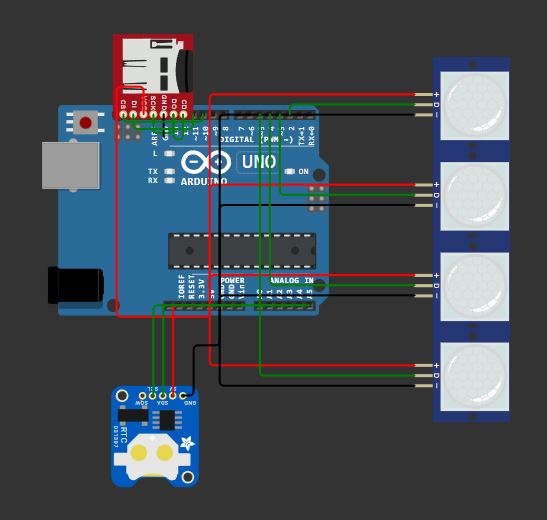
\includegraphics[width = 10cm]{ImagenesLatex/sensor4.JPG}{}
    \caption{Circuito 4 sensores PIR con reloj y SD}
    % \label{fig:enter-label}
\end{figure}

Y podemos utilizar Wokwi para simular el funcionamiento, ejemplo sin movimiento (inicio de simulación):
\begin{figure}[H]
    \centering
    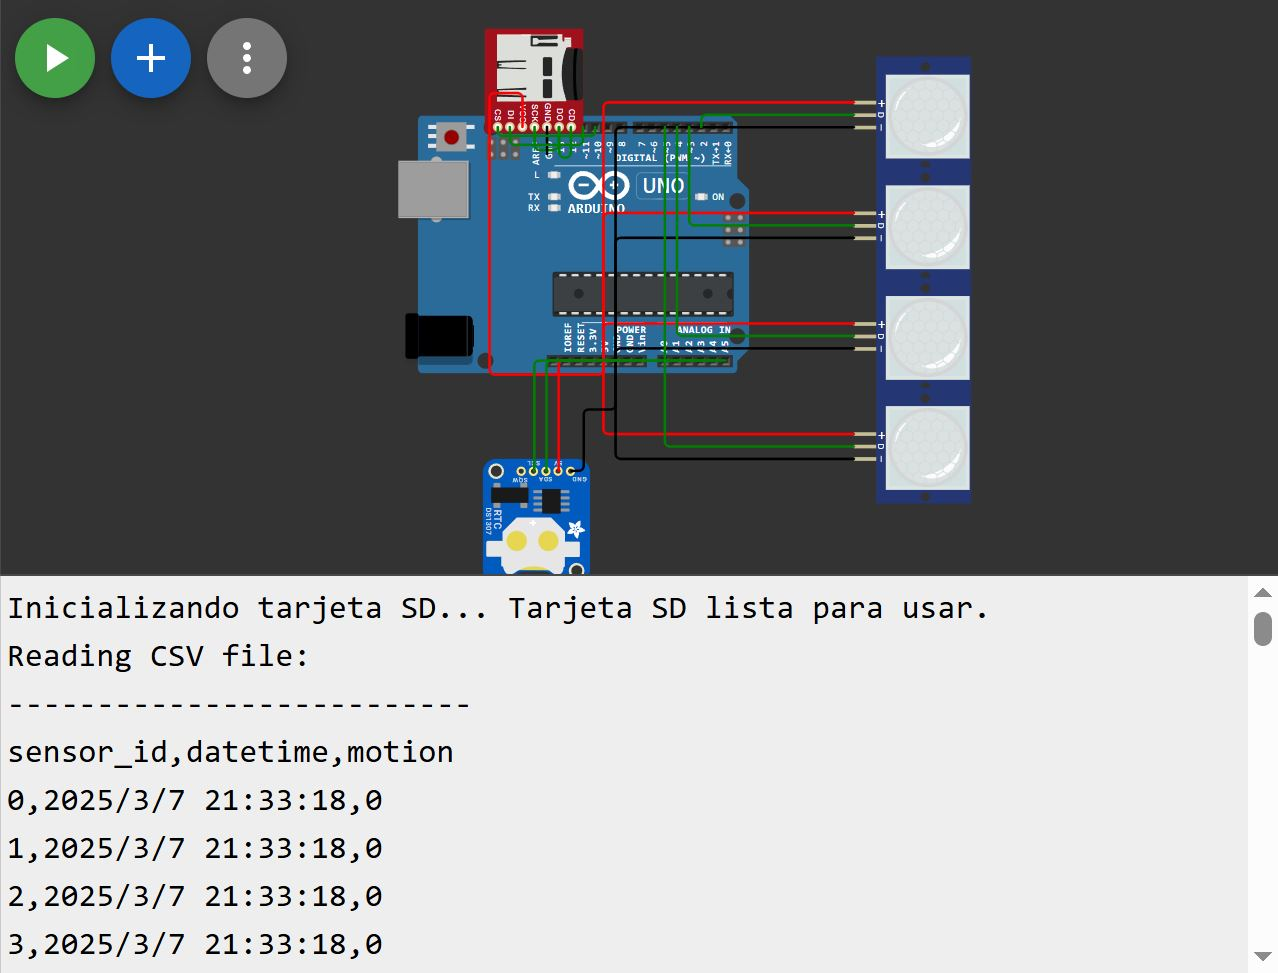
\includegraphics[width = 10cm]{ImagenesLatex/nomotion.JPG}{}
    \caption{Simulación 4 sensores PIR con reloj y SD (sin movimiento)}
    % \label{fig:enter-label}
\end{figure}

También podemos simular movimiento en el circuito, por ejemplo en el sensor de índice 2 que utiliza el pin 4 para lectura digital:

\begin{figure}[H]
    \centering
    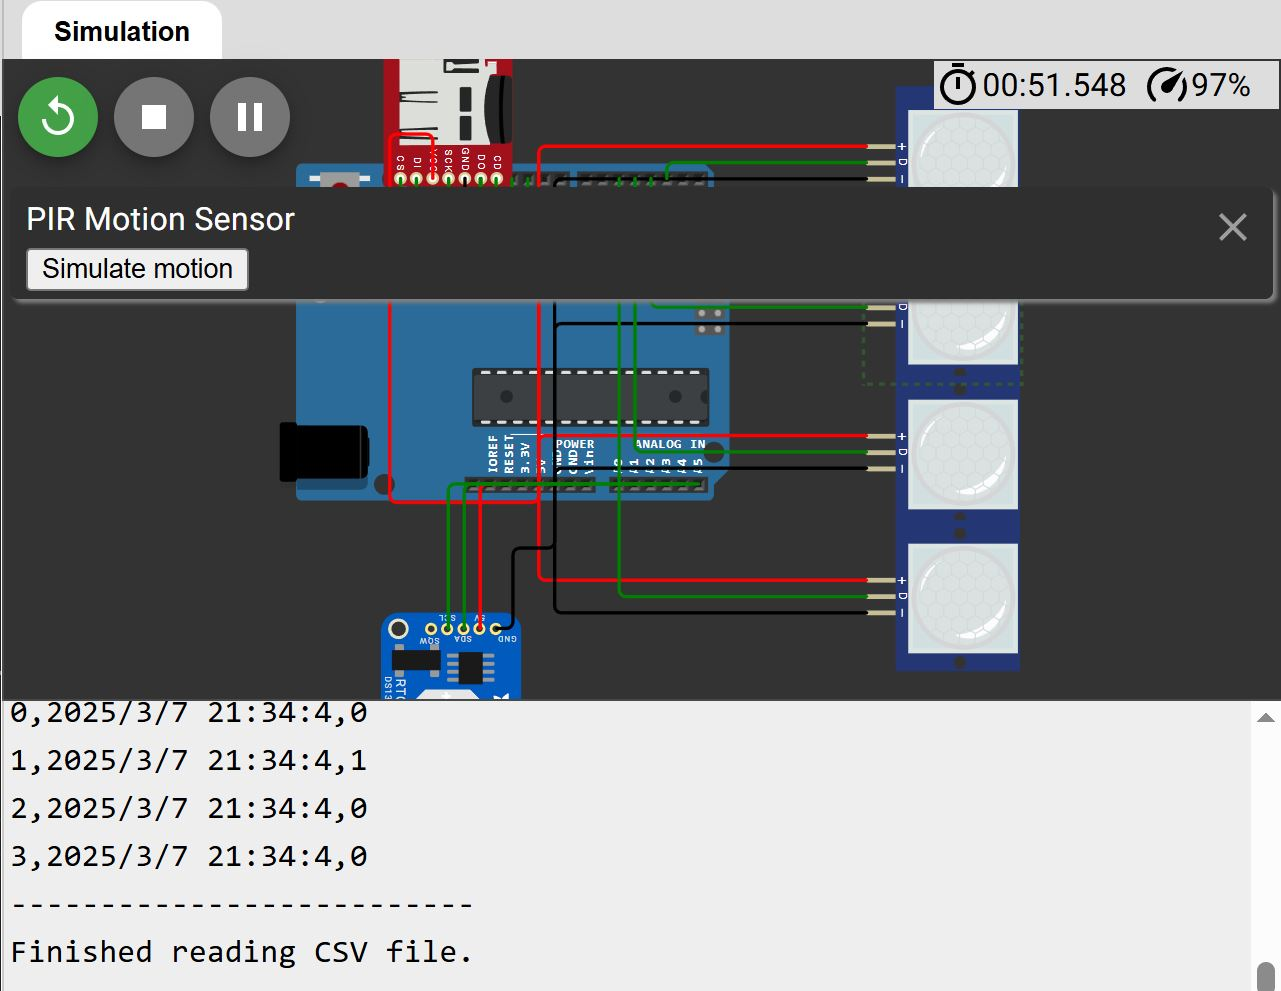
\includegraphics[width = 10cm]{ImagenesLatex/motion_s2.JPG}{}
    \caption{Simulación 4 sensores PIR con reloj y SD (movimiento sensor 2)}
    % \label{fig:enter-label}
\end{figure}

